\section{Background}

\subsection{The LUKS2 disk encryption specification}
also \cite{Fruwirth2018}

\emph{Linux Unified Key Setup 2}, or short LUKS2, is the second version of a disk encyption standard.
It provides a specification \cite{Broz2018} for a on-disk format for storing the encryption metadata as well as the encrypted
user data. Unlocking an encrypted disk is achieved by providing one of possibly multiple passphrases or keyfiles.
The intended usage of LUKS2 is together with the Linux dm-crypt subsystem, but that is not
mandatory\footnote{\label{fn:luks2windows} As we show in this thesis it is possible to make the combination of LUKS2 and
Windows work.}.

What are the differences between LUKS2 and LUKS? Besides new password hashing functions (I think)

Mention own \texttt{luks2} Rust crate

\begin{figure}
	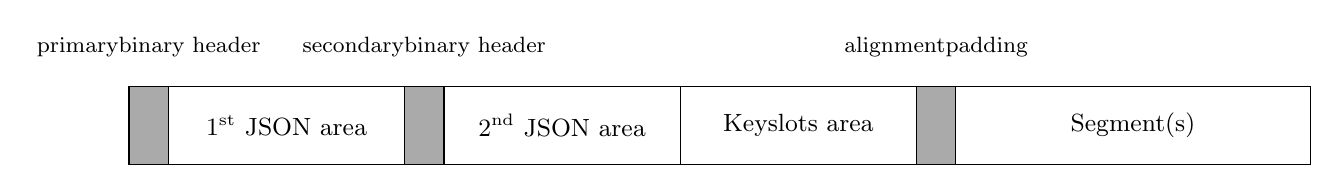
\begin{tikzpicture}
		\node [anchor=center] at (0.25, 1.5) {\footnotesize\makecell{primary\\binary header}};
		\draw [fill={rgb:black, 1; white, 2}] (0, 0) rectangle (0.5, 1);
		\draw [fill=white] (0.5, 0) rectangle (3.5, 1);
		\node [anchor=center] at (2, 0.5) {\small\makecell{1\textsuperscript{st} JSON area}};
		\node [anchor=center] at (3.75, 1.5) {\footnotesize\makecell{secondary\\binary header}};
		\draw [fill={rgb:black, 1; white, 2}] (3.5, 0) rectangle (4, 1);
		\draw [fill=white] (4, 0) rectangle (7, 1);
		\node [anchor=center] at (5.5, 0.5) {\small\makecell{2\textsuperscript{nd} JSON area}};
		\draw [fill=white] (7, 0) rectangle (10, 1);
		\node [anchor=center] at (8.5, 0.5) {\small\makecell{Keyslots area}};
		\node [anchor=center] at (10.25, 1.5) {\footnotesize\makecell{alignment\\padding}};
		\draw [fill={rgb:black, 1; white, 2}] (10, 0) rectangle (10.5, 1);
		\draw [fill=white] (10.5, 0) rectangle (15, 1);
		\node [anchor=center] at (12.75, 0.5) {\small\makecell{Segment(s)}};
	\end{tikzpicture}
	\caption{LUKS2 on-disk format (modified after \cite{Broz2018})}
	\label{fig:luks2ondisk}
\end{figure}

\subsection{Introduction to Windows kernel driver development}
This section gives an introduction on the development of Windows kernel drivers and related important concepts.

\subsubsection{Structure and Hierarchy of the Windows operating system}
Roughly summarize important concepts from chapters 1 and 2 of \cite{Yosifovich2017}

\subsubsection{The Windows Driver Model for kernel drivers}
Also explain how it gets loaded (if not done already)

\subsubsection{Communication between kernel and userspace}
Via ports